\section{Evaluación de Usabilidad}
\label{sec:eval_usabilidad}

La evaluación de la usabilidad consiste en realizar pruebas que proporcionen información con el propósito de identificar debilidades relacionadas al uso de las aplicaciones de software. Los objetivos de la evaluación pueden ser mejorar aspectos deficientes del software o realizar la comparación entre distintos software que ofrecen las mismas prestaciones. Las formas más comunes de evaluación son: automática (se registran datos y/o se calculan las métricas durante la ejecución de la aplicación), empírica (la usabilidad es evaluada testeando la aplicación con usuarios reales en laboratorios controlados), formal (usando modelos formales y fórmulas para el cálculo de medidas de usabilidad), e informal (basados en reglas generales y la habilidad y experiencia de los evaluadores). Los métodos no son excluyentes, la combinación de los mismos puede ofrecer información complementaria. El  proceso de evaluación implica varias actividades en función del método empleado, pero en general se agrupan en 3 pasos básicos: Captura de datos, Análisis y Crítica.
Desde las propuestas de Nielsen~\cite{NIELSEN1992} [4] hasta la actualidad, se han planteado una extensa y diversa cantidad de modelos y métricas para la evaluación de la usabilidad, por lo que en este trabajo no se proponen nuevas métricas. En su lugar se adoptará una propuesta que sirva al framework, que sea un modelo simple pero que puede escalar y sobre todo que haga eje en el concepto de tarea. El modelo de alto-nivel propuesto por Sauro y Kindlund~\cite{SK2005} [5] además de cumplir con las dimensiones ISO/ANSI (eficiencia, efectividad y satisfacción) logra sintetizar en cuatro métricas estas dimensiones y permite derivar otros indicadores útiles, como se ilustra en la Fig.~\ref{fig:fig1}. 

\begin{figure*}[ht!]
	\centering
	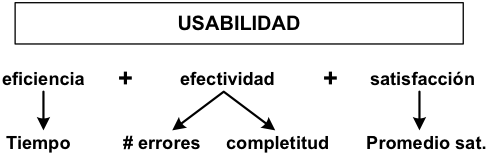
\includegraphics[scale=1]{figs/fig1.png}
	\caption{\label{fig:fig1} Modelo de Sauro y Kindlund~\cite{SK2005} \colorbox{green}{[4]}.}
\end{figure*}

%insertar fig1.png

La eficiencia se mide calculando el tiempo de la tarea, la efectividad se mide contabilizando el total de errores producidos durante la ejecución de la tarea y si ésta se ha completado. Por último, la satisfacción es un valor promedio obtenido de 3 ítems de valoración subjetivos, basados en una puntuación (1 a 5) que representan la complejidad de la tarea para el usuario, la satisfacción y la consideración del tiempo que le ha requerido dicha tarea). 
La propuesta de Sauro no incluye automatización del modelo, tal como indica en sus artículos, las pruebas fueron realizadas en laboratorios controlados en períodos de tiempo de dos años. 
